% Options for packages loaded elsewhere
% Options for packages loaded elsewhere
\PassOptionsToPackage{unicode}{hyperref}
\PassOptionsToPackage{hyphens}{url}
\PassOptionsToPackage{dvipsnames,svgnames,x11names}{xcolor}
%
\documentclass[
  letterpaper,
  DIV=11,
  numbers=noendperiod]{scrartcl}
\usepackage{xcolor}
\usepackage{amsmath,amssymb}
\setcounter{secnumdepth}{-\maxdimen} % remove section numbering
\usepackage{iftex}
\ifPDFTeX
  \usepackage[T1]{fontenc}
  \usepackage[utf8]{inputenc}
  \usepackage{textcomp} % provide euro and other symbols
\else % if luatex or xetex
  \usepackage{unicode-math} % this also loads fontspec
  \defaultfontfeatures{Scale=MatchLowercase}
  \defaultfontfeatures[\rmfamily]{Ligatures=TeX,Scale=1}
\fi
\usepackage{lmodern}
\ifPDFTeX\else
  % xetex/luatex font selection
\fi
% Use upquote if available, for straight quotes in verbatim environments
\IfFileExists{upquote.sty}{\usepackage{upquote}}{}
\IfFileExists{microtype.sty}{% use microtype if available
  \usepackage[]{microtype}
  \UseMicrotypeSet[protrusion]{basicmath} % disable protrusion for tt fonts
}{}
\makeatletter
\@ifundefined{KOMAClassName}{% if non-KOMA class
  \IfFileExists{parskip.sty}{%
    \usepackage{parskip}
  }{% else
    \setlength{\parindent}{0pt}
    \setlength{\parskip}{6pt plus 2pt minus 1pt}}
}{% if KOMA class
  \KOMAoptions{parskip=half}}
\makeatother
% Make \paragraph and \subparagraph free-standing
\makeatletter
\ifx\paragraph\undefined\else
  \let\oldparagraph\paragraph
  \renewcommand{\paragraph}{
    \@ifstar
      \xxxParagraphStar
      \xxxParagraphNoStar
  }
  \newcommand{\xxxParagraphStar}[1]{\oldparagraph*{#1}\mbox{}}
  \newcommand{\xxxParagraphNoStar}[1]{\oldparagraph{#1}\mbox{}}
\fi
\ifx\subparagraph\undefined\else
  \let\oldsubparagraph\subparagraph
  \renewcommand{\subparagraph}{
    \@ifstar
      \xxxSubParagraphStar
      \xxxSubParagraphNoStar
  }
  \newcommand{\xxxSubParagraphStar}[1]{\oldsubparagraph*{#1}\mbox{}}
  \newcommand{\xxxSubParagraphNoStar}[1]{\oldsubparagraph{#1}\mbox{}}
\fi
\makeatother


\usepackage{longtable,booktabs,array}
\newcounter{none} % for unnumbered tables
\usepackage{calc} % for calculating minipage widths
% Correct order of tables after \paragraph or \subparagraph
\usepackage{etoolbox}
\makeatletter
\patchcmd\longtable{\par}{\if@noskipsec\mbox{}\fi\par}{}{}
\makeatother
% Allow footnotes in longtable head/foot
\IfFileExists{footnotehyper.sty}{\usepackage{footnotehyper}}{\usepackage{footnote}}
\makesavenoteenv{longtable}
\usepackage{graphicx}
\makeatletter
\newsavebox\pandoc@box
\newcommand*\pandocbounded[1]{% scales image to fit in text height/width
  \sbox\pandoc@box{#1}%
  \Gscale@div\@tempa{\textheight}{\dimexpr\ht\pandoc@box+\dp\pandoc@box\relax}%
  \Gscale@div\@tempb{\linewidth}{\wd\pandoc@box}%
  \ifdim\@tempb\p@<\@tempa\p@\let\@tempa\@tempb\fi% select the smaller of both
  \ifdim\@tempa\p@<\p@\scalebox{\@tempa}{\usebox\pandoc@box}%
  \else\usebox{\pandoc@box}%
  \fi%
}
% Set default figure placement to htbp
\def\fps@figure{htbp}
\makeatother





\setlength{\emergencystretch}{3em} % prevent overfull lines

\providecommand{\tightlist}{%
  \setlength{\itemsep}{0pt}\setlength{\parskip}{0pt}}



 


\KOMAoption{captions}{tableheading}
\makeatletter
\@ifpackageloaded{caption}{}{\usepackage{caption}}
\AtBeginDocument{%
\ifdefined\contentsname
  \renewcommand*\contentsname{Table of contents}
\else
  \newcommand\contentsname{Table of contents}
\fi
\ifdefined\listfigurename
  \renewcommand*\listfigurename{List of Figures}
\else
  \newcommand\listfigurename{List of Figures}
\fi
\ifdefined\listtablename
  \renewcommand*\listtablename{List of Tables}
\else
  \newcommand\listtablename{List of Tables}
\fi
\ifdefined\figurename
  \renewcommand*\figurename{Figure}
\else
  \newcommand\figurename{Figure}
\fi
\ifdefined\tablename
  \renewcommand*\tablename{Table}
\else
  \newcommand\tablename{Table}
\fi
}
\@ifpackageloaded{float}{}{\usepackage{float}}
\floatstyle{ruled}
\@ifundefined{c@chapter}{\newfloat{codelisting}{h}{lop}}{\newfloat{codelisting}{h}{lop}[chapter]}
\floatname{codelisting}{Listing}
\newcommand*\listoflistings{\listof{codelisting}{List of Listings}}
\makeatother
\makeatletter
\makeatother
\makeatletter
\@ifpackageloaded{caption}{}{\usepackage{caption}}
\@ifpackageloaded{subcaption}{}{\usepackage{subcaption}}
\makeatother
\usepackage{bookmark}
\IfFileExists{xurl.sty}{\usepackage{xurl}}{} % add URL line breaks if available
\urlstyle{same}
\hypersetup{
  pdftitle={Credit Risk Modeling},
  pdfauthor={Munangiwa Gift Lithole},
  colorlinks=true,
  linkcolor={blue},
  filecolor={Maroon},
  citecolor={Blue},
  urlcolor={Blue},
  pdfcreator={LaTeX via pandoc}}


\title{Credit Risk Modeling}
\author{Munangiwa Gift Lithole}
\date{}
\begin{document}
\maketitle


\section{What is Credit Risk}

Credit risk is the risk a bank faces that a borrower may fail to meet
their contractual repayment obligations. Since lending is a core
activity of banks, this risk is significant because borrower defaults
can lead to financial losses, reduced profitability, and lower capital
adequacy.

To better understand and manage this risk, banks quantify it using
statistical and financial techniques. This process is known as
\textbf{credit risk modelling}, and it helps banks make decisions such
as whether to approve or reject loan applications.

\subsection{Credit Risk Metrics}

There are three key metrics used in credit risk modelling:

\begin{itemize}
\item
  \textbf{Probability of Default (PD):} This is the likelihood that a
  borrower will fail to meet their contractual repayment obligations. A
  default is commonly defined as the borrower missing payments for a
  specified period, often 90 days.
\item
  \textbf{Exposure at Default (EAD):} This is the total value the bank
  is exposed to at the time the borrower defaults. It includes the
  outstanding principal balance, accrued interest, and any applicable
  fees.
\item
  \textbf{Loss Given Default (LGD):} This is the percentage of the
  Exposure at Default that the bank cannot recover after taking
  collateral, guarantees, or recoveries into account.
\end{itemize}

These three metrics can be combined into a single measure known as the
\textbf{Expected Credit Loss (ECL):} \[ECL = PD \times EAD \times LGD\]
Conceptually, this formula represents the expected loss a bank may incur
from a loan due to borrower default.

\section{Techniques Used in Credit Risk Modeling}

Here, we focus on techniques used in modelling \textbf{Probability of
Default (PD)}.

There are two common types of PD measures: \textbf{Lifetime PD} and
\textbf{12-month PD}. However, our focus is on \textbf{12-month PD},
which measures the likelihood that a borrower will default within the
next 12 months after the loan has been approved.

The models used for PD estimation are typically \textbf{supervised
learning} models. This means that we train the models using historical
data where the outcomes are already known from past events. Since the
objective is to classify borrowers according to risk, PD modelling is
generally treated as a \textbf{classification problem}, where an
application is classified as either a \textbf{good borrower} or a
\textbf{bad borrower}.

Although these models produce probabilities, a threshold is selected to
convert the probabilities into classifications. A commonly used default
threshold is 0.50. Therefore:

\begin{itemize}
\tightlist
\item
  if the predicted probability of default is greater than or equal to
  0.50, the borrower may be classified as a bad borrower;
\item
  otherwise, the borrower is classified as a good borrower.
\end{itemize}

\[\text{Loan/Application} = \begin{cases} \text{Rejected/Default}, & \text{if } PD \geq 0.5 \\ \text{Approved/No Default}, & \text{if } PD < 0.5 \end{cases}\]

in a way the probalility represent risk, the higher the probability the
higher the risk of default

\subsection{Logistic Regression (Linear Model)}

Logistic Regression is a member of the \textbf{Generalized Linear Models
(GLM)} family, just like Linear Regression.

Both models examine the linear relationship between the
\textbf{independent variables} (features/inputs) and the
\textbf{dependent variable} (target/outcome). However, they differ in
the type of outcome they predict:

\begin{itemize}
\tightlist
\item
  \textbf{Linear Regression} is used when the outcome is a
  \textbf{continuous} variable.
\item
  \textbf{Logistic Regression} is used when the outcome is a
  \textbf{categorical} variable (typically binary: 0 or 1).
\end{itemize}

Logistic Regression predicts the \textbf{probability} of an event
occurring. This probability, denoted as \(p\), is bounded between
\textbf{0 and 1}.

If we tried to model \(p\) directly using a linear equation like we do
in linear regression:

\[p = \beta_0 + \beta_1 x_1 + \beta_2 x_2 + \dots + \beta_n x_n\]

we would run into serious problems. A linear model can produce any value
between \((-\infty, +\infty)\), but probability must stay within the
range \textbf{{[}0, 1{]}}. This makes direct modeling of probability
inappropriate.

Instead of modeling the probability \(p\) directly, we model the
\textbf{odds}:

\[
\text{odds} = \frac{p}{1 - p}
\]

where \(p\) is the probability of the event occurring.

Odds can take any value from \textbf{0 to +∞}. However, this range is
still not ideal for linear modeling because:

\begin{itemize}
\tightlist
\item
  It is not symmetric,
\item
  It cannot produce negative values.
\end{itemize}

To solve this, we take the \textbf{natural logarithm} of the odds. This
transformation gives us the \textbf{logit function} (also called
log-odds):

\[
\text{logit}(p) = \ln\left(\frac{p}{1-p}\right)
\]

The logit function has a very useful property: it maps probabilities
from (0, 1) to the entire real number line \textbf{(-∞, +∞)}. This makes
it suitable for linear modeling.

We can now assume a linear relationship between the \textbf{log-odds}
and the independent variables (features):

\[
\ln\left(\frac{p}{1-p}\right) = \beta_0 + \beta_1 x_1 + \beta_2 x_2 + \dots + \beta_n x_n
\]

where:

\begin{itemize}
\tightlist
\item
  \(x_1, x_2, \dots, x_n\) are the input features,
\item
  \(\beta_0, \beta_1, \dots, \beta_n\) are the model coefficients
  (parameters).
\end{itemize}

We can rearrange the equation to express the probability \$ p \$
directly:

\[
p = \frac{1}{1 + e^{-(\beta_0 + \beta_1 x_1 + \beta_2 x_2 + \dots + \beta_n x_n)}}
\]

This is known as the \textbf{sigmoid function} (or logistic function):

\[
\sigma(z) = \frac{1}{1 + e^{-z}}
\]

where \(z = \beta_0 + \beta_1 x_1 + \dots + \beta_n x_n\) is the linear
combination of the features.

By applying the sigmoid function to the linear predictor, we obtain a
valid probability that always lies between \textbf{0 and 1}.

\begin{figure}[H]

{\centering 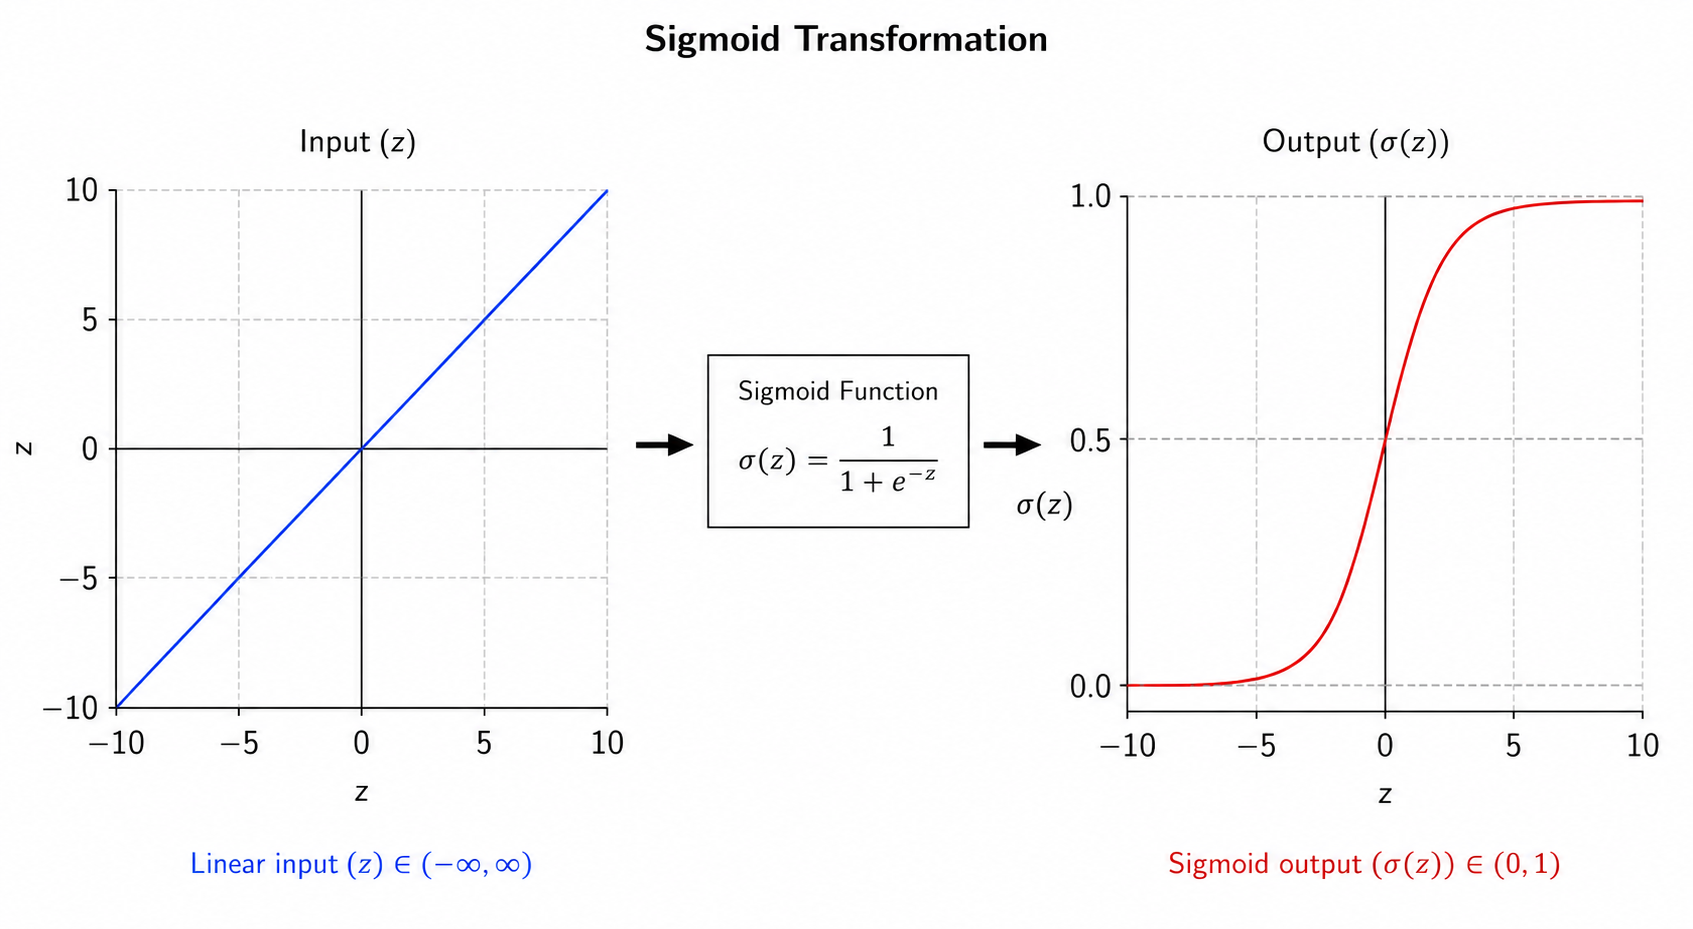
\includegraphics[width=0.7\linewidth,height=\textheight,keepaspectratio]{sigmoid.png}

}

\caption{Sigmoid Transformation}

\end{figure}%

\subsection{Tree-Based Models (Non-Linear)}

These are non-parametric supervised learning algorithms that use a
hierarchical tree-like structure to make predictions. The algorithms
recursively split the features to find optimal split points that best
separate the data and improve the prediction of event probabilities.

Tree-based models are particularly useful for capturing non-linear
relationships and interactions between variables without requiring
strict statistical assumptions.(\textbf{No mathematical equations})

\begin{itemize}
\tightlist
\item
  \textbf{Decision Tree}: This model consists of a single tree used to
  make predictions.
\item
  \textbf{Random Forest}: This model consists of many decision trees
  used for prediction, where the final prediction is typically obtained
  by averaging the predictions from all the trees.
\item
  \textbf{Gradient Boosting Machine}: This model also uses many trees;
  however, each new tree is built to learn from and correct the mistakes
  made by the previous trees, improving the overall predictive
  performance.
\end{itemize}

\begin{figure}[H]

{\centering 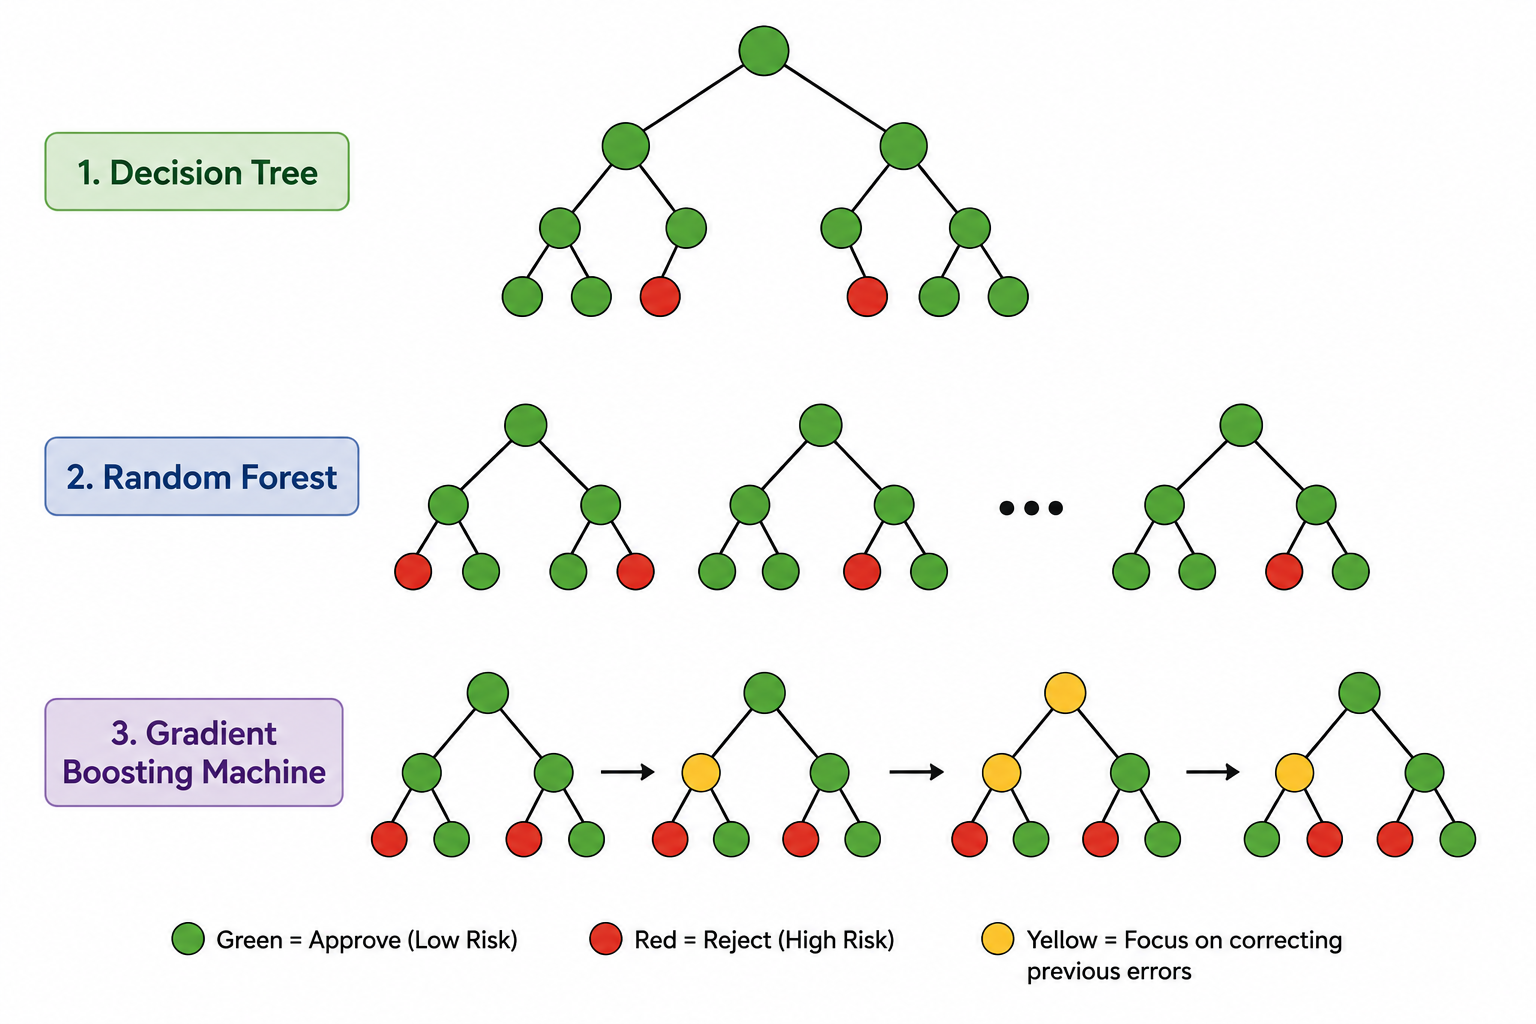
\includegraphics[width=0.7\linewidth,height=\textheight,keepaspectratio]{trees.png}

}

\caption{Tree Base Model}

\end{figure}%

\subsection{Neural Networks (Non-Linear)}

A neural network is a machine learning model that stacks simple
computational units called \emph{neurons} in multiple layers. These
neurons learn patterns in the data by estimating weights and biases that
map inputs to outputs.

At a high level, neural networks are inspired by biological neurons in
the human brain, which communicate through electrical signals.

The structure of an artificial feed-forward neural network can be
represented by the recursive expression:
\[\mathbf{a}^{(l)} = \sigma_l\left(\mathbf{W}_l^T \mathbf{a}^{(l-1)} + \mathbf{b}^{(l)}\right), \quad l = 1,2,\dots,L\]
where:

\begin{itemize}
\tightlist
\item
  \(\mathbf{a}^{(l)}\) is the vector of activation values at layer
  \(l\),
\item
  \(\mathbf{W}_l\) is the weight matrix for layer \(l\),
\item
  \(\mathbf{b}^{(l)}\) is the bias vector for layer \(l\),
\item
  and \(\sigma_l\) is the activation function applied at layer \(l\).
\end{itemize}

The initial layer, \(\mathbf{a}^{(0)}\), represents the input features
for a particular observation, usually denoted by:

\[
\mathbf{a}^{(0)} = \mathbf{x}_i
\]

Just like in logistic regression, the \textbf{activation function}
applied at the final layer (L) (the output layer) is typically the
sigmoid function when dealing with binary classification problems.

The sigmoid activation function maps the output to a value between 0 and
1, allowing it to be interpreted as a probability of default.

\begin{figure}[H]

{\centering 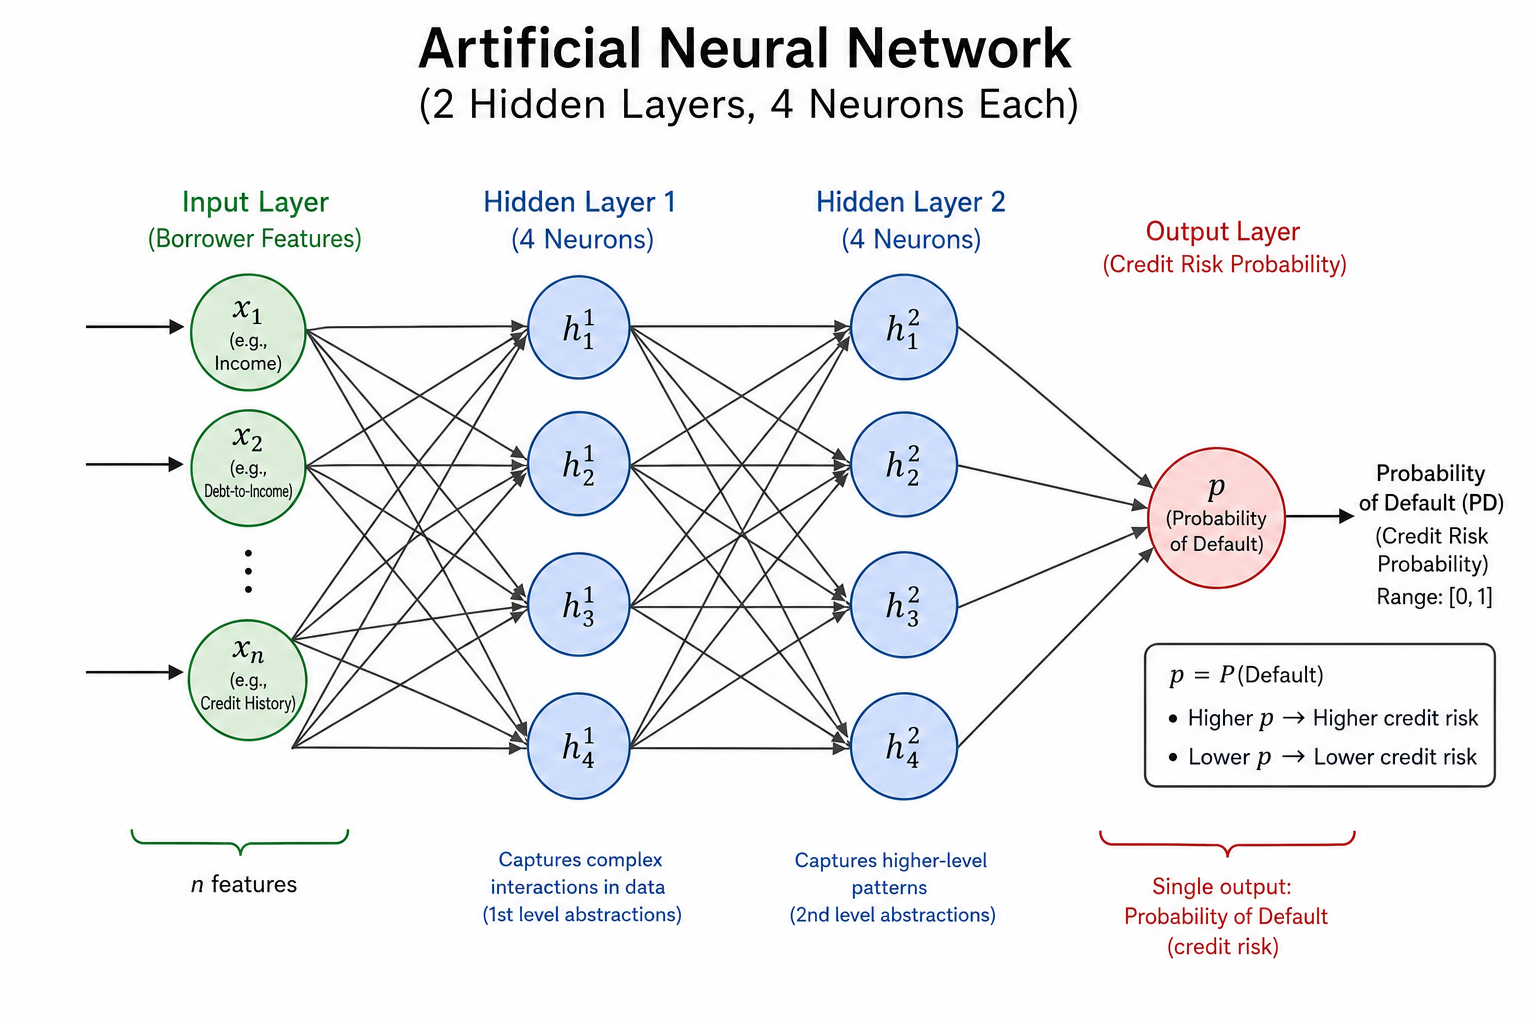
\includegraphics[width=0.7\linewidth,height=\textheight,keepaspectratio]{neural.png}

}

\caption{Artificial Neural Network}

\end{figure}%

\subsection{Others(Non-Linear)}

The following are other methods that can also be used:

\begin{itemize}
\tightlist
\item
  Support vector machine
\item
  K-Nearest Neighbors (KNN)
\item
  Naïve Bayes
\end{itemize}

\subsection{Complexity and Interpretability}

So we can see that logistic regression and decision trees are simple
models and do not involve many complicated processes that we can lose
track of. This means that these models are interpretable. However, they
are not very strong at capturing complex structures.

We also see that in random forests, gradient boosting machines, and
neural networks, many processes are involved before reaching a
prediction. Therefore, it is easier to lose track of how predictions are
made, making these models less interpretable. However, these models are
strong at capturing complex structures.

\subsection{Weights of Evidence(WoE) and Information Value (IV)}

\begin{itemize}
\tightlist
\item
  \textbf{Weight of Evidence (WoE):} It is a measure of the strength of
  a feature (independent variable) in separating non-events and events.
  In our case, it measures how well a feature can separate good and bad
  loan applications.
\end{itemize}

\[\text{WoE}_i = \ln\left(\frac{\% \text{ of non-events}_i}{\% \text{ of events}_i}\right)
= \ln\left(\frac{\text{Distribution of Good}_i}{\text{Distribution of Bad}_i}\right)\]

\(i\) is refer to the ith bin/category

\begin{itemize}
\tightlist
\item
  \textbf{Information Value (IV):} It is used to measure the predictive
  power of independent variables. It helps us understand which
  independent variables provide the most useful information about the
  target variable. IV is commonly used as a variable selection technique
  when the dependent variable (target) is binary, meaning it has only
  two possible values.
\end{itemize}

\[
\text{IV} = \sum_{i=1}^{n} \left( \text{WoE}_i \times \left( \% \text{ of non-events}_i - \% \text{ of events}_i \right) \right)\]

So, \textbf{Weight of Evidence (WoE)} is important in credit modelling
because we typically use \textbf{logistic regression}, which assumes a
linear relationship between the \textbf{log-odds of the target variable}
and the input features.

In practice, WoE is mainly applied to \textbf{categorical variables (or
continuous variables that have been binned into categories)}. It
transforms these categories into numerical values that are linearly
related to the log-odds of the target. This makes the features more
suitable for logistic regression and improves both model stability and
interpretability.

WoE is also useful because it groups categories that have similar
distributions with respect to the target variable. This allows us to
rank risk across categories by observing how the default rate changes
from one group to another.

Ideally, we want this relationship to be \textbf{monotonic} (either
consistently increasing or consistently decreasing), meaning that risk
should move in a single direction across the ordered categories. This
makes the model more interpretable and aligned with credit risk
intuition.

\subsection{Model Evaluation Metrics}

So, the \textbf{positive class} is the event we are modelling, which is
a bad loan application (default), and the \textbf{negative class}
represents the non-event, which is a good loan application
(non-default).

Many metrics that follow are defined from the \textbf{confusion matrix}:

\begin{itemize}
\tightlist
\item
  \textbf{True Positive (TP):} The actual event is default, and the
  model predicts default.
\item
  \textbf{False Negative (FN):} The actual event is default, however the
  model predicts non-default.
\item
  \textbf{False Positive (FP):} The actual event is non-default, however
  the model predicts default.
\item
  \textbf{True Negative (TN):} The actual event is non-default, and the
  model predicts non-default.
\end{itemize}

\begin{table}[h]
\centering
\begin{tabular}{c|cc}
\hline
 & \textbf{Predicted Positive} & \textbf{Predicted Negative} \\
\hline
\textbf{Actual Positive} & TP & FN \\
\textbf{Actual Negative} & FP & TN \\
\hline
\end{tabular}
\caption{Confusion Matrix}
\end{table}

\begin{enumerate}
    \item \textbf{Accuracy}: This is the overall percentage of correct predictions. It measures how many of the total predictions made by the model were correct, whether default or non-default.

    $$
    \text{Accuracy} = \frac{\text{TP + TN}}{\text{TP + FP + FN + TN}}
    $$

   \item \textbf{Precision}: This measures how well the model predicts defaults (the positive class). Out of all loan applications predicted to default, it shows how many actually defaulted.

    $$
    \text{Precision} = \frac{\text{TP}}{\text{TP + FP}}
    $$

    \item \textbf{Recall}: This measures how well the model identifies all actual default events. Out of all loan applications that actually defaulted, it shows how many the model correctly predicted as default.

    $$
    \text{Recall} = \frac{\text{TP}}{\text{TP + FN}}
    $$

    \item \textbf{F1 Score}: This is the harmonic mean of Precision and Recall. It is used to balance the trade-off between the two. For example, if one model has high precision and another has high recall, the F1 score helps identify a balance between them and can be used to compare models.

    \item \textbf{AUC (Area Under the Curve)}: This refers to the area under the Receiver Operating Characteristic (ROC) curve. The ROC curve shows how well the model separates default (events) from non-default (non-events) across all possible classification thresholds used to define an event.

    \item \textbf{Gini}: This also measures how well the model separates defaults and non-defaults. It is directly related to AUC:

    $$
    \text{Gini} = 2 \times \text{AUC} - 1
    $$


\end{enumerate}

\section{Forbidden Features}

The features that a regulator will disapprove of are primarily those
that introduce discrimination and those that lack business
interpretability.

\textbf{Forbidden features} include race, religion, gender, marital
status, etc. They also include \textbf{proxy variables} of such
attributes---features that are indirectly correlated with protected
characteristics, such as zip code, geographical data, email domain, etc.

These features are disallowed because of fair lending practices. Models
must not perpetuate bias or discrimination, and they must also support
explainability and accountability, since lenders are required to provide
clear reasons when rejecting a loan application.

\section{Data Cleaning Approach}

The dataset (loan book) contains \textbf{602 duplicate records}, which
will be removed.

There are \textbf{4 variables} with missing values:

\begin{itemize}
    \item annual\_income: 8638
    \item employment\_length\_years: 3711
    \item num\_open\_accounts: 2423
    \item months\_since\_last\_delinquency: 60068
\end{itemize}

The variable \textbf{months\_since\_last\_delinquency} was dropped
because nearly half of its observations contain missing values.

For \textbf{annual\_income}, the data was grouped by region, and the
missing values were imputed using the median annual income within each
region. The reason for this approach is that income levels may differ
across locations.

For \textbf{employment\_length\_years} and \textbf{num\_open\_accounts},
missing values were imputed using the median of each variable.

The variables \textbf{age}, \textbf{employment\_length\_years},
\textbf{num\_open\_accounts}, and
\textbf{months\_since\_oldest\_account} had float data types, although
they should be stored as integers. In addition,
\textbf{application\_date} had a string (object) data type instead of a
date format.

The data types were converted to their appropriate formats.

It was also observed that the variables \textbf{home\_ownership} and
\textbf{loan\_purpose} contained inconsistent label formatting. The
category labels were standardized to ensure consistency.

\section{Exploratory Data Analysis(EDA)}

\begin{figure}[H]

{\centering 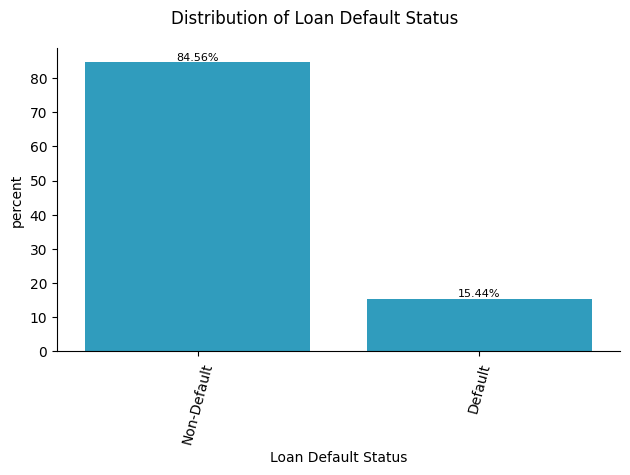
\includegraphics[width=0.7\linewidth,height=\textheight,keepaspectratio]{Target.png}

}

\caption{Target Distribution}

\end{figure}%

We start by looking at the \textbf{target distribution}. From the target
distribution diagram, we can see that people who defaulted make up
15.44\% of the dataset, while non-defaults account for 84.56\%. This
shows that the dataset is imbalanced and further implies that there are
many good customers and relatively few bad customers.

\begin{figure}[H]

{\centering 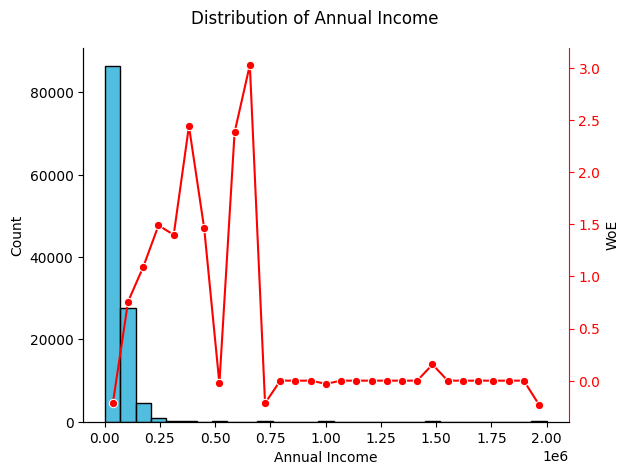
\includegraphics[width=0.7\linewidth,height=\textheight,keepaspectratio]{annual_income.png}

}

\caption{Annual Income}

\end{figure}%

Next, we consider the histogram of annual income. From the histogram, we
can observe that there are many tall bars on the left side and fewer
bars spread across the right side. This indicates that annual income is
right-skewed (has a long right tail) and may contain potential outliers.
This suggests that most people earn lower incomes, while only a few
people earn very high incomes.

Now consider the WoE plot (shown in red). We can observe that the red
line generally increases from one bin to another, indicating that the
risk of default decreases as annual income increases. Although the
relationship is not perfectly monotonic, this is likely because some
bins at the higher income levels contain very few customers. For
example, if a bin contains only one customer and that customer
defaulted, the WoE value may fluctuate significantly. This explains why
the red line becomes unstable in the later bins.

\begin{figure}[H]

{\centering 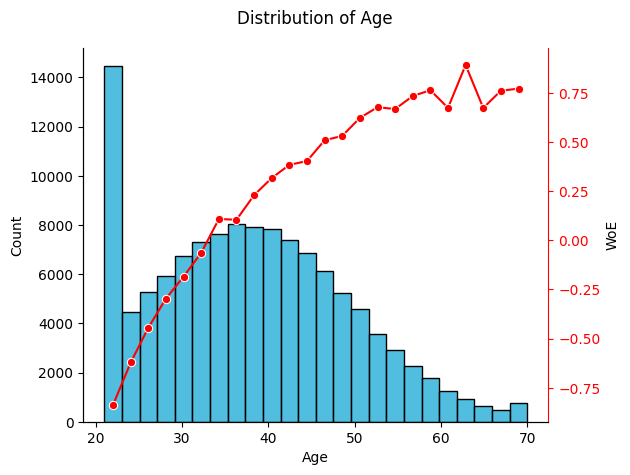
\includegraphics[width=0.7\linewidth,height=\textheight,keepaspectratio]{age.png}

}

\caption{Age}

\end{figure}%

The histogram for age appears approximately normally distributed, with a
larger concentration of younger applicants around age 21. The WoE plot
(red line) is consistently increasing, showing the monotonic
relationship that we expect. However, the curve increases at a
decreasing rate, suggesting a non-linear relationship between age and
the log-odds of default.

The increasing WoE trend indicates that as age increases, the risk of
default decreases. This suggests that younger applicants are generally
more likely to default than older applicants.

\begin{figure}[H]

{\centering 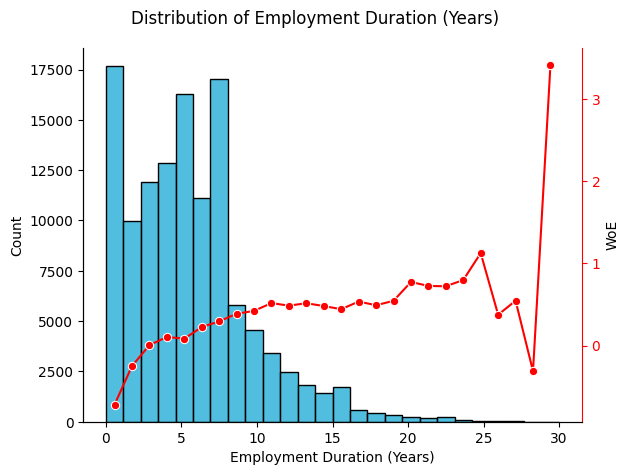
\includegraphics[width=0.7\linewidth,height=\textheight,keepaspectratio]{employ.png}

}

\caption{Employment Duration (Years)}

\end{figure}%

For employment duration, the histogram shows a slight right tail, with
most people having employment durations between 0 and 10 years. The WoE
plot (red line) generally increases, although it is not perfectly
monotonic. The curved shape suggests that employment duration is not
perfectly linearly related to the log-odds.

The increasing trend implies that as employment duration increases, the
risk of default decreases. This suggests that early-career professionals
are generally more likely to default compared to more experienced
individuals.

\begin{figure}[H]

{\centering 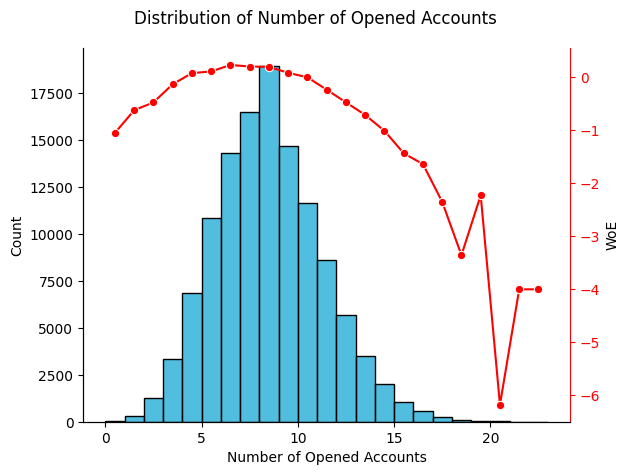
\includegraphics[width=0.7\linewidth,height=\textheight,keepaspectratio]{num_open.png}

}

\caption{Number of Opened Accounts}

\end{figure}%

The histogram for the number of opened accounts appears approximately
normally distributed, with most people having around 8 opened accounts.
The WoE plot forms a quadratic-like shape, suggesting that the variable
does not have a linear relationship with the log-odds, but rather a
non-linear relationship.

This indicates that when customers have very few accounts, opening
additional accounts may initially reduce risk. However, after reaching
approximately 8 accounts, the risk of default begins to increase again
as more accounts are opened. This suggests that both very low and very
high numbers of opened accounts may be associated with higher default
risk, although having too many accounts appears riskier.

\begin{figure}[H]

{\centering 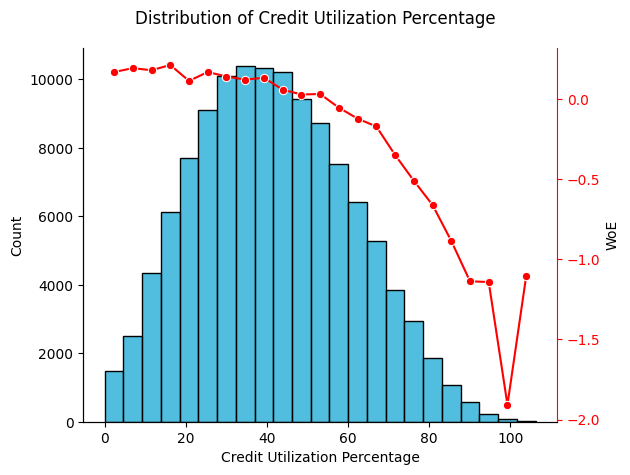
\includegraphics[width=0.7\linewidth,height=\textheight,keepaspectratio]{credit_util.png}

}

\caption{Credit Utilisation Percentage}

\end{figure}%

The distribution of credit utilisation percentage appears approximately
normally distributed, with many customers using around 41\% of their
available credit. The WoE plot is consistently decreasing, showing a
monotonic relationship, although it is not perfectly linear because the
curve is slightly curved.

The decreasing WoE trend indicates that as credit utilisation increases,
the risk of default also increases. This implies that customers who use
a smaller proportion of their available credit are generally less risky
than those with high credit utilisation.

\begin{figure}[H]

{\centering 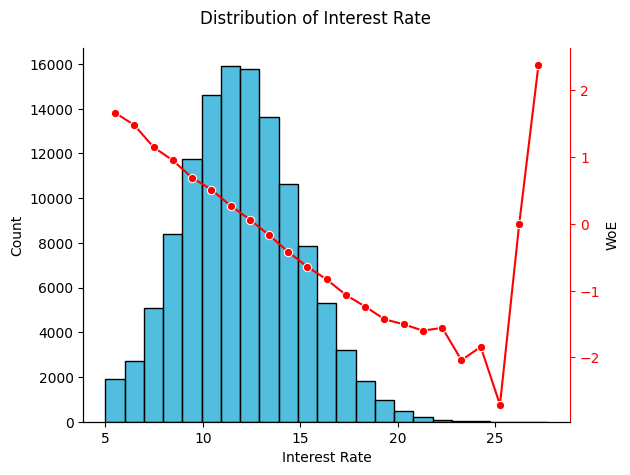
\includegraphics[width=0.7\linewidth,height=\textheight,keepaspectratio]{interest.png}

}

\caption{Interest Rate}

\end{figure}%

For interest rate, the distribution appears approximately normal, with
most customers being charged around a 12\% interest rate. The WoE plot
generally decreases, which is the monotonic relationship we expect,
although there is some zig-zag behaviour at the extreme bins that may be
due to potential outliers.

This suggests that interest rate has a relatively linear relationship
with the log-odds of default. We can further conclude that higher
interest rates are associated with a higher risk of default. In other
words, when loans become less affordable, borrowers are more likely to
default.

\begin{figure}[H]

{\centering 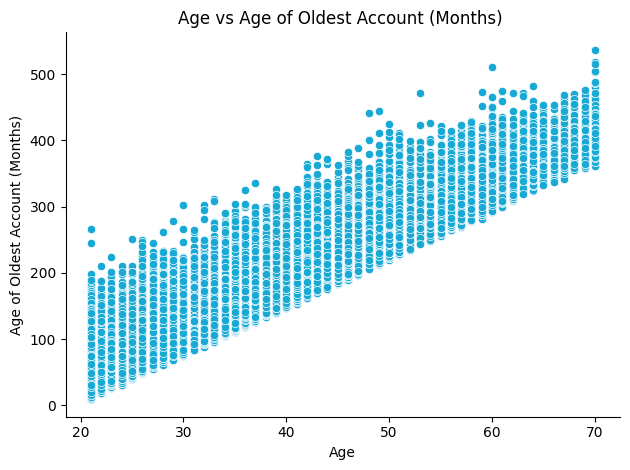
\includegraphics[width=0.7\linewidth,height=\textheight,keepaspectratio]{age_vs_older.png}

}

\caption{Age vs Months Since The Oldest Account}

\end{figure}%

Age is positively and linearly related to months since the oldest
account. This means that older individuals tend to have older credit
accounts. The relationship suggests a strong correlation between the two
variables.

\section{Feature Engineering Choices}

For feature engineering, we first consider \textbf{annual\_income}.
Since the variable was right-skewed and contained potential outliers, a
new variable called \texttt{log\_annual\_income\_capped} was created.
First, the \texttt{annual\_income} variable was capped to reduce the
effect of extreme outliers, and then a logarithmic transformation was
applied to the capped values. The logarithmic transformation helps
improve the relationship between annual income and the log-odds by
making the relationship more linear. the variables
\texttt{total\_revolving\_balance} and \texttt{loan\_amount} where also
applied logarithmic transformation.

For the variables \texttt{age}, \texttt{num\_open\_accounts},
\texttt{credit\_utilisation\_pct}, and
\texttt{employment\_length\_years}, the exploratory data analysis showed
that these features had non-linear relationships with the log-odds of
default. To better capture these relationships, new transformed
variables ending with \texttt{\_WoE} were created, for example
\texttt{feature\_WoE}.

For each variable, the values were separated into bins, and each
observation was replaced with the corresponding Weight of Evidence (WoE)
value for the bin to which it belonged. This transformation helps
capture non-linear relationships while also making the variables more
suitable for logistic regression.

\section{Modeling Methodology}

For this credit risk model, logistic regression was selected as the
primary modelling technique. The main reason for choosing logistic
regression is that it is highly interpretable and suitable for binary
classification problems, where the objective is to distinguish between
good and bad customers by predicting the likelihood of default.

In addition, logistic regression produces predicted probabilities, which
can be used to support lending decisions such as whether to approve or
reject a loan application.

The dataset was split into training and testing sets using the variable
named \texttt{set} in the data. The training set contains 70\% of the
observations, while the testing set contains the remaining 30\%.

A baseline logistic regression model was first fitted after removing all
forbidden features. Thereafter, additional engineered features were
added one at a time to evaluate whether they improved model performance.
This process continued until all newly engineered features had been
assessed.

The primary objective during model development was to improve the
model's \textbf{AUC (Area Under the ROC Curve)}, since AUC measures how
well the model distinguishes between default and non-default borrowers.

\section{Final Logistic Regression Model}

The final logistic regression model obtained is and variables where
scaled:

\[
\begin{aligned}
\log\left(\frac{p}{1-p}\right) =\;& -0.4299 \\
&-0.5754(\text{log\_annual\_income\_capped}) \\
&+0.5387(\text{num\_delinquencies\_2yr}) \\
&-0.3895(\text{age\_woe}) \\
&-0.3275(\text{num\_open\_accounts\_woe}) \\
&+0.2715(\text{num\_hard\_inquiries\_6mo}) \\
&-0.2678(\text{credit\_utilisation\_pct\_woe}) \\
&-0.2371(\text{employment\_length\_years\_woe}) \\
&+0.1012(\text{dti\_ratio}) \\
&-0.0907(\text{pct\_accounts\_current}) \\
&-0.0246(\text{log\_total\_revolving\_balance})\\
&+0.0179(\text{log\_loan\_amount})
\end{aligned}\]

The estimated intercept of the model is:

\[
\beta_0 = -0.4299\]

The odds ratios corresponding to each coefficient are shown below:

\[
\begin{array}{lcc}
\hline
\textbf{Feature} & \textbf{Coefficient} & \textbf{Odds Ratio} \\
\hline
\text{log\_annual\_income\_capped} & -0.5754 & 0.562 \\
\text{num\_delinquencies\_2yr} & 0.5387 & 1.714 \\
\text{age\_woe} & -0.3895 & 0.677 \\
\text{num\_open\_accounts\_woe} & -0.3275 & 0.721 \\
\text{num\_hard\_inquiries\_6mo} & 0.2715 & 1.312 \\
\text{credit\_utilisation\_pct\_woe} & -0.2678 & 0.765 \\
\text{employment\_length\_years\_woe} & -0.2371 & 0.789 \\
\text{dti\_ratio} & 0.1012 & 1.107 \\
\text{pct\_accounts\_current} & -0.0907 & 0.913 \\
\text{log\_total\_revolving\_balance} & -0.0246 & 0.976 \\
\text{log\_loan\_amount} &  0.0179 & 1.018  \\
\hline
\end{array}\]

\section{Interpretation of the Final Logistic Regression Model}

Since the variables were scaled before fitting the logistic regression
model, the coefficients represent the effect of a one standard deviation
increase in each feature on the log-odds of default, holding all other
variables constant.

The odds ratios describe the multiplicative change in the odds of
default associated with a one standard deviation increase in a feature.

\begin{itemize}

    \item \textbf{log\_annual\_income\_capped} has a negative coefficient ($-0.5754$) and an odds ratio of $0.562$. This indicates that higher income is associated with lower default risk. A one standard deviation increase in this variable decreases the odds of default by approximately $43.8\%$.

    \item \textbf{num\_delinquencies\_2yr} has a positive coefficient ($0.5387$) and an odds ratio of $1.714$. This suggests that borrowers with more past delinquencies are more likely to default. A one standard deviation increase in this feature increases the odds of default by approximately $71.4\%$.

    \item \textbf{age\_woe} has a negative coefficient ($-0.3895$), indicating that borrowers in lower-risk age groups are generally less likely to default.

    \item \textbf{num\_open\_accounts\_woe} has a negative coefficient ($-0.3275$), suggesting that favourable account structures are associated with lower default risk.

    \item \textbf{num\_hard\_inquiries\_6mo} has a positive coefficient ($0.2715$) and an odds ratio of $1.312$. This indicates that borrowers with more recent hard inquiries are more likely to default.

    \item \textbf{credit\_utilisation\_pct\_woe} has a negative coefficient ($-0.2678$), showing that lower-risk credit utilisation groups are associated with lower default probabilities.

    \item \textbf{employment\_length\_years\_woe} has a negative coefficient ($-0.2371$), suggesting that stronger employment profiles are associated with lower default risk.

    \item \textbf{dti\_ratio} has a positive coefficient ($0.1012$), indicating that higher debt-to-income ratios are associated with increased default risk.

    \item \textbf{pct\_accounts\_current} has a negative coefficient ($-0.0907$), implying that borrowers with a higher proportion of current accounts are generally less risky.

    \item \textbf{log\_total\_revolving\_balance} has a positive coefficient ($-0.0246$), suggesting that higher total revolving balance are associated with lowering default risk.

    \item \textbf{log\_loan\_amount} has a positive coefficient ($0.0179$), suggesting that larger loan amounts slightly increase default risk.

\end{itemize}

\section{Performance Relative to Baseline}

The current logistic regression model achieved an AUC of 0.79,
outperforming the baseline logistic regression model (AUC = 0.68).

\begin{itemize}
\item
  Absolute improvement: +0.11
\item
  Relative improvement: +16.18\% over the baseline
\end{itemize}




\end{document}
